\documentclass[a4paper,12pt]{report}
\usepackage[utf8]{inputenc}
\usepackage{graphicx}
\usepackage{hyperref}
\usepackage{textcomp}
\usepackage{mathtools}

\begin{document}
\begin{titlepage}
\begin{center}
    \vspace*{1cm}
    
    \Huge
    \textbf{Computer Music Languages and Systems}
    
    \vspace{0.5cm}
    \LARGE
    Homework n° 2\\
   	Flanger effect plugin with feedback

    \vspace{1 cm}
    
    \textbf{10574752}
    
    \vspace{0.5cm}
    
    \textbf{10751438}
     
    \vspace{0.5cm}
    
    \textbf{10612929}
     
    
    \vspace{0.5cm}
    
    \textbf{10486570}
    
    \vspace{0.5cm}
    
    \vfill
  
   
    \date{May 2021}
    \vspace{0.3cm}
    \textbf{Master of Science in Music and Acoustic Engineering}
    
    \vspace{0.8cm}
    
    
\includegraphics[width=0.5\textwidth]{logo_positivo.png}
    
\end{center}
\end{titlepage}


\abstract{}
Our group worked on \textbf{Assignment 3}: implement a 			  	flanger effect plugin with feedback. We divided our work in 		 	steps as presented in the sections of this document. After a quick theory recap about the behaviour of a flanger unit with feedback, we chose the parameters that best suit for a flanger plugin. Finally, we got our hands on JUCE, implementing the code behind the functionality of these parameters and the Graphical User Interface.
In general, we used as a reference the "Material on delay lines" PDF document and the related JUCE laboratories, expecially the Delay Line one.
Here is the link to the GitHub Repository containing all the code: \url{https://github.com/EllDy96/CarlGang/tree/Homework2}
\endabstract{}

\chapter{}
\section{Theory recap: flanger with feedback}
Flanger is a delay-based effect. So, we started from the implementation of the \textbf{Delay Line}, considering that the amount of the delay varies over time, under the control of a separate \textbf{Low-Frequency Oscillator} \textbf{(LFO)}. Moreover, adding a \textbf{feedback control}, the output of the delay line is routed back to its input. %This causes the sound to repeat continuously, and assuming a feedback gain less than 1, the echoes will become quieter each time. Though the echoes are theoretically repeated forever, they will eventually become so quiet as to be below the ambient noise in the system and thus be inaudible.
\\In the picture below a block diagram of a flanger with feedback unit is shown:
\begin{figure}[h]
\centering
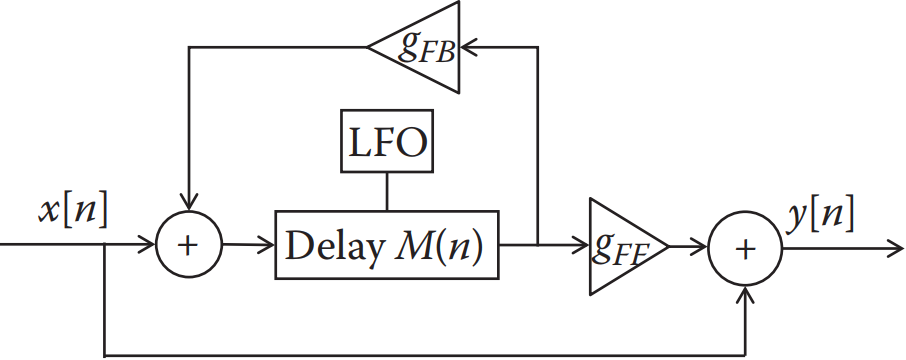
\includegraphics[scale=.45]{db_flanger.png}
\caption{Flanger with feedback}
\end{figure}
\\As we can see from the block diagram, we have two gains, $\textit{g}_{FB}$, which is the feedback gain, and $\textit{g}_{FF}$, the gain related to the output of the delay line. If $\textit{g}_{FB}<1$, the delayed copies of the sound will gradually decay, where a gain of 1 or more means they will grow indefinitely.
So, the input/output relation for the flanger with feedback can be expressed in the time domain as:
\[ y[n] = x[n]+ g_{FF}d[n]\] where $d[n]=x[n-M[n]]+g_{FB}d[n-M[n]] $ is the output of the delay line. $M[n]$ expresses the delay length over a sample $n$. There are different $M$ functions, depending on the particular waveform we are using. Generally, we can describe $M$ through the following parameters: 
\begin{itemize}
\item[\textperiodcentered] $M_{0}$ (in samples), the delay given by the delay control;
\item[\textperiodcentered] $M_{W}$ (in samples), the delay given by the sweep width control; 
\item[\textperiodcentered] $\phi$, the phase of the waveform (in rad).
\end{itemize}
For our plugin we are going to use the following waveforms, with $\phi \in [0,1]$:
\begin{itemize}
\item[\textperiodcentered] Sine: \[ M(\phi) = M_{0}+M_{W}(\frac{1}{2}+\frac{1}{2}\sin(2\pi \phi))\] 
\item[\textperiodcentered] Triangle:
  \begin{equation}
    M(\phi) =
    \begin{cases*}
      M_{0} + M_{W}(\frac{1}{2}+2\phi) & if $0\leq \phi<\frac{1}{2}$ \\
      M_{0} + M_{W}(1-2(\phi-1/4)) & if $\frac{1}{2}\leq \phi<\frac{3}{4}$ \\
      M_{0} + 2M_{W}(\phi-\frac{3}{4}) & if $\frac{3}{4}\leq \phi\leq 1$
    \end{cases*}
\end{equation}
\item[\textperiodcentered] Sawtooth:
  \begin{equation}
    M(\phi) =
    \begin{cases*}
      M_{0} + M_{W}(\frac{1}{2}+\phi) & if $\phi\leq \frac{1}{2}$\\
      M_{0} + M_{W}(\phi-\frac{1}{2}) & if $\frac{1}{2}<\phi\leq 1$
    \end{cases*}
\end{equation}
\end{itemize}
\section{Parameters choice}
The parameters we chose for our flanger plugin are the following:
\begin{itemize}
\item \textbf{Feedforward (Mix)} $\rightarrow$ \textsc{knob}
\\It represents the amount of delayed signal that is mixed in with the original one. Having a value of 0 means that we are considering only the dry signal. Increasing this value (up to 1), one can adjust the balance between the processed signal and the dry signal.
\item \textbf{Feedback} $\rightarrow$ \textsc{knob}
\\Through this parameter it's possible to control, in practice, how much of the output signal from the delay line we want to send back through the device input. The range of possible values for this plugin is $[0, 0.50]$. We decided to set the end of the range at half of his theoretical maximum because the more it approaches 1 the more emerges a metallic sound due to the sharpening of peaks and notches in the frequency response.
\item \textbf{Delay} $\rightarrow$ \textsc{knob}
\\It lets the user to adjust the minimum amount of delay of the LFO, in a range of $[1.00, 5.00]$[ms]. For higher delay times our flanger behaved as a chorus, so we fixed the max at 5 ms.
\item \textbf{LFO Width (Sweep Width)} $\rightarrow$ \textsc{knob}
\\It allows one to control the total amplitude of waveform of the LFO, in a range of $[1.00, 20.00]$[ms].
\item \textbf{LFO Frequency (Speed)} $\rightarrow$ \textsc{knob}
\\The LFO frequency can be set in a range of $[0.05, 2.00]$[Hz].
\item \textbf{Shape of the LFO Envelope} $\rightarrow$ \textsc{Combo Box}
\\It allows one to select which shape use for the LFO. For this plugin there are three possible waveform shapes: Sine, Triangle and Sawtooth.
\end{itemize}

%\begin{table}[!h]
%\centering
%\begin{tabular}{|c|c|c|}
%\hline
%           & \begin{tabular}[c]{@{}c@{}}Train\\ (\# elem)\end{tabular} & \begin{tabular}[c]{@{}c@{}}Test\\ (\# elem)\end{tabular} \\ \hline
%Distortion & 1394                                                      & 1238                                                     \\ \hline
%Tremolo    & 1194                                                      & 1228                                                     \\ \hline
%NoFX       & 559                                                       & 555                                                      \\ \hline
%\end{tabular}
%\caption{Train and test datasets sizes}
%\label{tab:my-table}
%\end{table}

\section{Plugin implementation in JUCE}
\subsection{Processor implementation}
\begin{itemize}
\item[\textasteriskcentered]The first thing we decided to implement is the Value Tree State, a class used to manage all the parameters of the plugin, or so to say, the entire plugin’s state. It is very helpful in order to handle the connection between the objects in the Editor and the Processor via the instantiation of specific classes called Attachments, one for each type of graphical objects (i.e., slider, comboBox). An identification string is used for retrieving a parameter, and by using the Value Tree State, the post-condition of the get method ensures that the parameter is the newest value up to date with the user interface.  
\item[\textasteriskcentered] As a delay-based effect, the flanger is implemented using circular buffers, which can be considered as FIFO buffers (First In First Out). The dimension of the buffer is fixed and it is large enough to fit the amount of the maximum delay (sweep width + delay parameters) at any point in the LFO cycle.
\\The actual length of delay at any time is controlled by the distance between the read pointer and the write pointer in the buffer. The increase or decrease of the delay is represented by the speed of the read pointer with respect to the movement of the write pointer. If the read pointer moves faster (slower), the amount of delay will decrease (increase).
\item[\textasteriskcentered] In addition, we need to use low order polynomial interpolation to calculate the output of the delay line, including the case in which the delay length, expressed by the function M[n], is not an integer. First, we tried to implement a simple linear interpolation, but then we opted instead for the cubic interpolation because the former was causing some artefacts. In either case, we left the linear interpolation commented in the code for a quick comparison. 
\item[\textasteriskcentered] In order to handle the multiple waveforms of the LFO, we defined the wave functions through a switch case in which the phase varies incrementally. Given the wave functions, it easy to compute the current delay with the user-defined parameters width and delay and hence the delay read pointer:
\begin{verbatim}
float currentDelay = delay + sweepWidth * waveformFunction;
\end{verbatim}
\end{itemize}
\subsection{GUI implementation}
In order to create the knobs, we created two custom classes (BlueKnobStyle,MagentaKnobStyle)\footnote{The classes are exactly the same except the colour of the smaller circle} in the \emph{PluginEditor.h} that use the juce method \textbf{LookAndFeel\_V4}. The class draw the knob starting from a rotary slider, drawing two concentric circles and rotating a rectangle using the method juce::AffineTransform. Then we defined two elements (blueKnob,mageKnob) of the classes in the AudioProcessorEditor that gives the style defined to the slider using the function \emph{setLookAndFeel} in the editor compiler.

\chapter{}
\section{Result and Demo}
To recreate the famous "jet passing overhead" characteristic sound of the flanger, we recorded a clean guitar and applied some distortion (adding higher frequencies enhance the effect). And finally, we fed the guitar recording to delay with the following parameters:
\begin{itemize}
\item \textbf{Feedforward} $= 1$
\item \textbf{Feedback} $= 0.25$
\item \textbf{Delay} $= 1$ ms
\item \textbf{LFO Width} $= 4.5$ ms 
\item \textbf{LFO Freq} $= 0.1$ Hz
\item \textbf{Waveform} = sine
\end{itemize}

The result can be played at the following link:\\ \verb"inserire link"


\newpage
We also include the start-up window of the plugin with all the default parameters:
\begin{figure}[h]
\centering
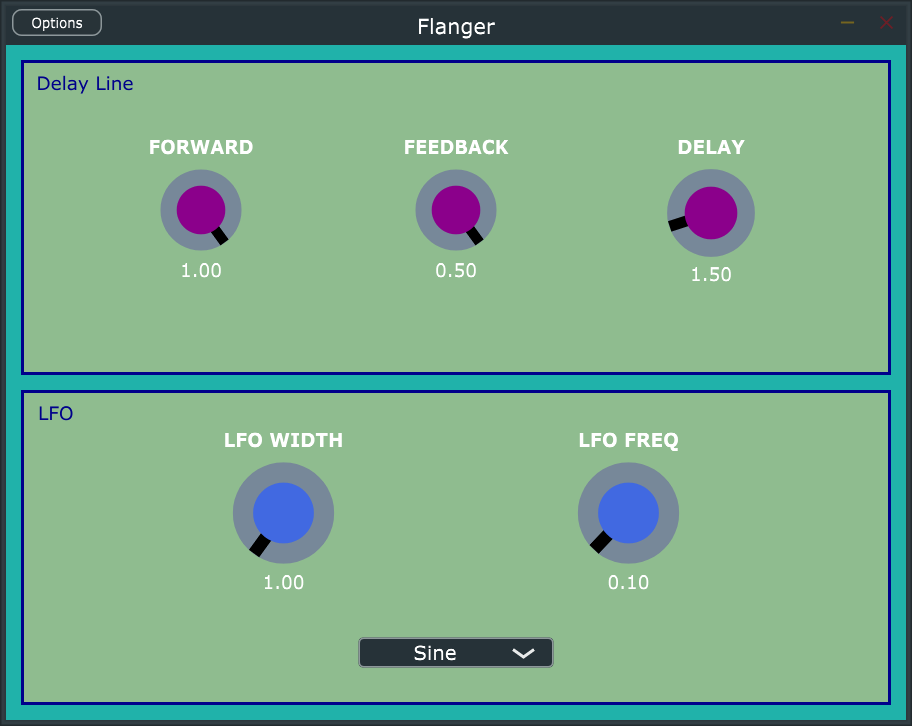
\includegraphics[scale=0.75]{ui.png}
\caption{User interface}
\end{figure}








\end{document}
